% Options for packages loaded elsewhere
\PassOptionsToPackage{unicode}{hyperref}
\PassOptionsToPackage{hyphens}{url}
%
\documentclass[
]{article}
\usepackage{amsmath,amssymb}
\usepackage{iftex}
\ifPDFTeX
  \usepackage[T1]{fontenc}
  \usepackage[utf8]{inputenc}
  \usepackage{textcomp} % provide euro and other symbols
\else % if luatex or xetex
  \usepackage{unicode-math} % this also loads fontspec
  \defaultfontfeatures{Scale=MatchLowercase}
  \defaultfontfeatures[\rmfamily]{Ligatures=TeX,Scale=1}
\fi
\usepackage{lmodern}
\ifPDFTeX\else
  % xetex/luatex font selection
\fi
% Use upquote if available, for straight quotes in verbatim environments
\IfFileExists{upquote.sty}{\usepackage{upquote}}{}
\IfFileExists{microtype.sty}{% use microtype if available
  \usepackage[]{microtype}
  \UseMicrotypeSet[protrusion]{basicmath} % disable protrusion for tt fonts
}{}
\makeatletter
\@ifundefined{KOMAClassName}{% if non-KOMA class
  \IfFileExists{parskip.sty}{%
    \usepackage{parskip}
  }{% else
    \setlength{\parindent}{0pt}
    \setlength{\parskip}{6pt plus 2pt minus 1pt}}
}{% if KOMA class
  \KOMAoptions{parskip=half}}
\makeatother
\usepackage{xcolor}
\usepackage[margin=1in]{geometry}
\usepackage{color}
\usepackage{fancyvrb}
\newcommand{\VerbBar}{|}
\newcommand{\VERB}{\Verb[commandchars=\\\{\}]}
\DefineVerbatimEnvironment{Highlighting}{Verbatim}{commandchars=\\\{\}}
% Add ',fontsize=\small' for more characters per line
\usepackage{framed}
\definecolor{shadecolor}{RGB}{248,248,248}
\newenvironment{Shaded}{\begin{snugshade}}{\end{snugshade}}
\newcommand{\AlertTok}[1]{\textcolor[rgb]{0.94,0.16,0.16}{#1}}
\newcommand{\AnnotationTok}[1]{\textcolor[rgb]{0.56,0.35,0.01}{\textbf{\textit{#1}}}}
\newcommand{\AttributeTok}[1]{\textcolor[rgb]{0.13,0.29,0.53}{#1}}
\newcommand{\BaseNTok}[1]{\textcolor[rgb]{0.00,0.00,0.81}{#1}}
\newcommand{\BuiltInTok}[1]{#1}
\newcommand{\CharTok}[1]{\textcolor[rgb]{0.31,0.60,0.02}{#1}}
\newcommand{\CommentTok}[1]{\textcolor[rgb]{0.56,0.35,0.01}{\textit{#1}}}
\newcommand{\CommentVarTok}[1]{\textcolor[rgb]{0.56,0.35,0.01}{\textbf{\textit{#1}}}}
\newcommand{\ConstantTok}[1]{\textcolor[rgb]{0.56,0.35,0.01}{#1}}
\newcommand{\ControlFlowTok}[1]{\textcolor[rgb]{0.13,0.29,0.53}{\textbf{#1}}}
\newcommand{\DataTypeTok}[1]{\textcolor[rgb]{0.13,0.29,0.53}{#1}}
\newcommand{\DecValTok}[1]{\textcolor[rgb]{0.00,0.00,0.81}{#1}}
\newcommand{\DocumentationTok}[1]{\textcolor[rgb]{0.56,0.35,0.01}{\textbf{\textit{#1}}}}
\newcommand{\ErrorTok}[1]{\textcolor[rgb]{0.64,0.00,0.00}{\textbf{#1}}}
\newcommand{\ExtensionTok}[1]{#1}
\newcommand{\FloatTok}[1]{\textcolor[rgb]{0.00,0.00,0.81}{#1}}
\newcommand{\FunctionTok}[1]{\textcolor[rgb]{0.13,0.29,0.53}{\textbf{#1}}}
\newcommand{\ImportTok}[1]{#1}
\newcommand{\InformationTok}[1]{\textcolor[rgb]{0.56,0.35,0.01}{\textbf{\textit{#1}}}}
\newcommand{\KeywordTok}[1]{\textcolor[rgb]{0.13,0.29,0.53}{\textbf{#1}}}
\newcommand{\NormalTok}[1]{#1}
\newcommand{\OperatorTok}[1]{\textcolor[rgb]{0.81,0.36,0.00}{\textbf{#1}}}
\newcommand{\OtherTok}[1]{\textcolor[rgb]{0.56,0.35,0.01}{#1}}
\newcommand{\PreprocessorTok}[1]{\textcolor[rgb]{0.56,0.35,0.01}{\textit{#1}}}
\newcommand{\RegionMarkerTok}[1]{#1}
\newcommand{\SpecialCharTok}[1]{\textcolor[rgb]{0.81,0.36,0.00}{\textbf{#1}}}
\newcommand{\SpecialStringTok}[1]{\textcolor[rgb]{0.31,0.60,0.02}{#1}}
\newcommand{\StringTok}[1]{\textcolor[rgb]{0.31,0.60,0.02}{#1}}
\newcommand{\VariableTok}[1]{\textcolor[rgb]{0.00,0.00,0.00}{#1}}
\newcommand{\VerbatimStringTok}[1]{\textcolor[rgb]{0.31,0.60,0.02}{#1}}
\newcommand{\WarningTok}[1]{\textcolor[rgb]{0.56,0.35,0.01}{\textbf{\textit{#1}}}}
\usepackage{longtable,booktabs,array}
\usepackage{calc} % for calculating minipage widths
% Correct order of tables after \paragraph or \subparagraph
\usepackage{etoolbox}
\makeatletter
\patchcmd\longtable{\par}{\if@noskipsec\mbox{}\fi\par}{}{}
\makeatother
% Allow footnotes in longtable head/foot
\IfFileExists{footnotehyper.sty}{\usepackage{footnotehyper}}{\usepackage{footnote}}
\makesavenoteenv{longtable}
\usepackage{graphicx}
\makeatletter
\def\maxwidth{\ifdim\Gin@nat@width>\linewidth\linewidth\else\Gin@nat@width\fi}
\def\maxheight{\ifdim\Gin@nat@height>\textheight\textheight\else\Gin@nat@height\fi}
\makeatother
% Scale images if necessary, so that they will not overflow the page
% margins by default, and it is still possible to overwrite the defaults
% using explicit options in \includegraphics[width, height, ...]{}
\setkeys{Gin}{width=\maxwidth,height=\maxheight,keepaspectratio}
% Set default figure placement to htbp
\makeatletter
\def\fps@figure{htbp}
\makeatother
\setlength{\emergencystretch}{3em} % prevent overfull lines
\providecommand{\tightlist}{%
  \setlength{\itemsep}{0pt}\setlength{\parskip}{0pt}}
\setcounter{secnumdepth}{-\maxdimen} % remove section numbering
\ifLuaTeX
  \usepackage{selnolig}  % disable illegal ligatures
\fi
\usepackage{bookmark}
\IfFileExists{xurl.sty}{\usepackage{xurl}}{} % add URL line breaks if available
\urlstyle{same}
\hypersetup{
  pdftitle={Ayudantía 1},
  pdfauthor={Equipo Estadística 2},
  hidelinks,
  pdfcreator={LaTeX via pandoc}}

\title{Ayudantía 1}
\author{Equipo Estadística 2}
\date{2025-03-11}

\begin{document}
\maketitle

\subsection{Ayudantías}\label{ayudantuxedas}

•Las ayudantías serán semanales y con asistencia.

•Tendrán un enfoque en el refuerzo práctico de los contenidos de clase.

•Habrá controles en las ayudantías; estos no serán complejos y la idea
es que puedan reforzar lo visto en clase.

\subsection{Fechas}\label{fechas}

\begin{itemize}
\item
  Control AyudaLab 1: 27/03/2025
\item
  Control AyudaLab 2: 17/04/2025
\item
  Control AyudaLab 3: 22/05/2025
\item
  Control AyudaLab 4: 05/06/2025
\item
  Control AyudaLab 5: 03/07/2025
\end{itemize}

**Finalmente, la idea es que a lo largo de las ayudantías del curso,
podamos desarrollar un Libro R que sirva de repositorio de los
principales códigos utilizados.

\subsection{Contenidos Ayudantía 1}\label{contenidos-ayudantuxeda-1}

•Esta primera ayudantía tiene la finalidad de repasar los elementos
centrales de R, para eso veremos lo siguiente:

\begin{enumerate}
\def\labelenumi{\arabic{enumi}.}
\tightlist
\item
  Qué es R y RStudio
\item
  Interfaz RStudio
\item
  Funciones básicas
\item
  Vectores y bbdd
\item
  Trabajo en R
\item
  Paquetes
\item
  BBDD
\end{enumerate}

\subsection{R y Rstudio}\label{r-y-rstudio}

•Existen múltiples programas para el análisis estadístico, siendo los
más populares STATA, SPSS y R. R se ha vuelto el software más utilizado
en los últimos años, debido a su accesibilidad gratuita, su potencia en
análisis/presentación de información y su versatilidad por ser de código
abierto. (Eso y muchas otras razones)

•R es el programa/lenguaje de programación y Rstudio es un entorno que
actúa como interfaz para hacer más amigable la utilización y navegación
por R.

•Si bien el programa se utiliza en mayor medida para análisis
estadístico, también tiene gran potencialidad en análisis cualitativos,
presentación de información, entre muchas otras funciones.

\subsection{R y Rstudio}\label{r-y-rstudio-1}

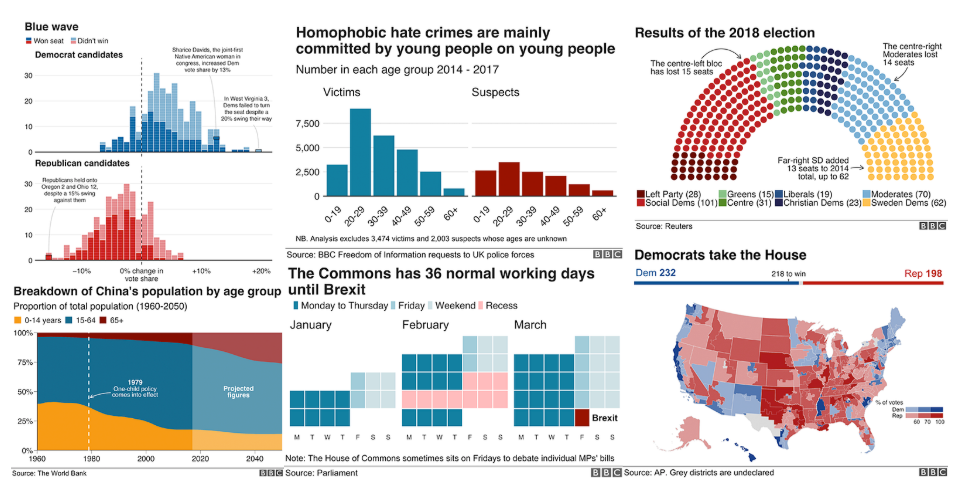
\includegraphics[width=5.625in,height=\textheight]{GrafR.png}

\subsection{R y Rstudio}\label{r-y-rstudio-2}

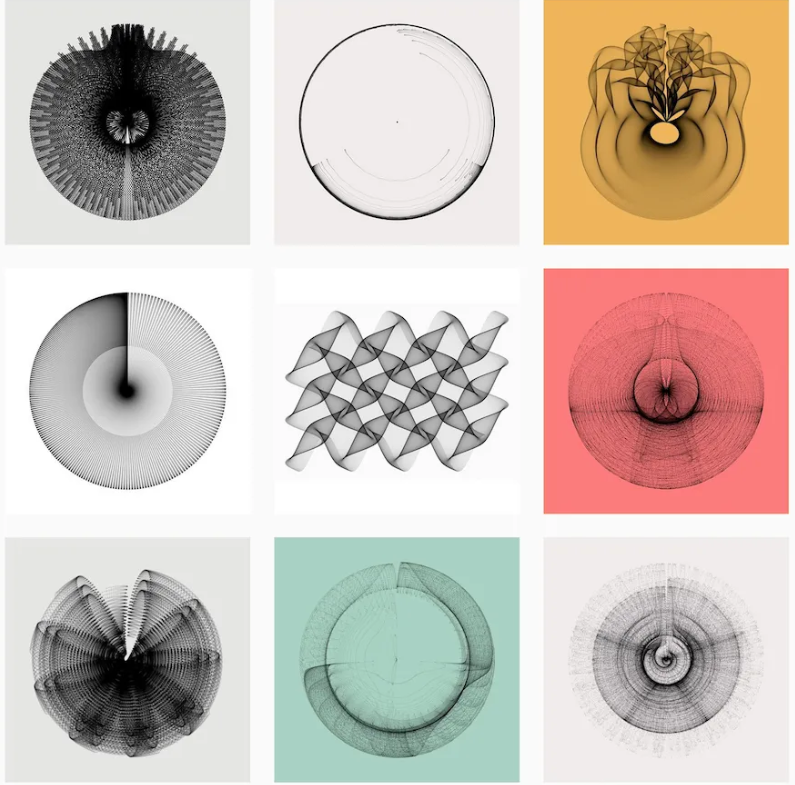
\includegraphics[width=3.03125in,height=\textheight]{ArteR.png}

\subsection{Rstudio}\label{rstudio}

\includegraphics{Presentación Proyecto libreta Creativo Doodle Rosa.jpg}

\subsection{Funciones básicas en R}\label{funciones-buxe1sicas-en-r}

•Como bien recordarán, podemos utilizar R para realizar operaciones
básicas:

\begin{Shaded}
\begin{Highlighting}[]
\DecValTok{300}\SpecialCharTok{+}\DecValTok{200}
\end{Highlighting}
\end{Shaded}

\begin{verbatim}
## [1] 500
\end{verbatim}

\begin{Shaded}
\begin{Highlighting}[]
\DecValTok{100{-}42}
\end{Highlighting}
\end{Shaded}

\begin{verbatim}
## [1] 58
\end{verbatim}

\begin{Shaded}
\begin{Highlighting}[]
\DecValTok{4}\SpecialCharTok{*}\DecValTok{7}
\end{Highlighting}
\end{Shaded}

\begin{verbatim}
## [1] 28
\end{verbatim}

\begin{Shaded}
\begin{Highlighting}[]
\DecValTok{25}\SpecialCharTok{/}\DecValTok{5}
\end{Highlighting}
\end{Shaded}

\begin{verbatim}
## [1] 5
\end{verbatim}

•También nos permite establecer comparaciones entre valores:

\begin{Shaded}
\begin{Highlighting}[]
\DecValTok{100} \SpecialCharTok{==} \DecValTok{200} \CommentTok{\# "==" Esto significa igual a}
\end{Highlighting}
\end{Shaded}

\begin{verbatim}
## [1] FALSE
\end{verbatim}

\begin{Shaded}
\begin{Highlighting}[]
\DecValTok{400} \SpecialCharTok{\textgreater{}} \DecValTok{399} \CommentTok{\# Mayor a}
\end{Highlighting}
\end{Shaded}

\begin{verbatim}
## [1] TRUE
\end{verbatim}

\subsection{Funciones básicas en R}\label{funciones-buxe1sicas-en-r-1}

•Además de la adición, sustracción, multiplicación y división, estas son
otras funciones básicas en R

\begin{longtable}[]{@{}ll@{}}
\toprule\noalign{}
Operación & Significado \\
\midrule\noalign{}
\endhead
\bottomrule\noalign{}
\endlastfoot
== & Igual a \\
!= & Distinto a \\
\textgreater{} & Mayor que \\
\textgreater= & Mayor o igual que \\
\textless{} & Menor que \\
\textless= & Menor o igual que \\
\end{longtable}

•Estas se vuelven importantes cuando queramos recodificar y filtrar
variables.

\subsection{Vectores}\label{vectores}

•Los vectores son conjuntos de datos del mismo tipo, aplicado a las
ciencias sociales estos serían variables. Podemos destacar 3 tipos de
vectores más relevantes:

\begin{enumerate}
\def\labelenumi{\arabic{enumi}.}
\item
  Numéricos: valores numéricos, incluye decimales.
\item
  Carácter: valores alfanuméricos, es decir, letras, números y signos
  mezclados.
\item
  Lógicos: valores lógicos. (TRUE o FALSE)
\end{enumerate}

\subsection{Vectores}\label{vectores-1}

•Para la creación de vectores se debe utilizar la función concatenar.

•En el caso de vectores numéricos, los números decimales se deben
escribir con un ``.'', ya que, la coma (``,'') es la que indica
separación de valores.

\begin{Shaded}
\begin{Highlighting}[]
\NormalTok{estaturas }\OtherTok{\textless{}{-}} \FunctionTok{c}\NormalTok{(}\FloatTok{1.85}\NormalTok{, }\FloatTok{1.63}\NormalTok{, }\FloatTok{1.75}\NormalTok{, }\FloatTok{1.57}\NormalTok{)}
\end{Highlighting}
\end{Shaded}

•En los vectores de carácter, las palabras deben ir entre comillas
(``\,``)

\begin{Shaded}
\begin{Highlighting}[]
\NormalTok{nombres }\OtherTok{\textless{}{-}} \FunctionTok{c}\NormalTok{(}\StringTok{"Ana"}\NormalTok{, }\StringTok{"Alejandro"}\NormalTok{, }\StringTok{"Andrés"}\NormalTok{, }\StringTok{"María"}\NormalTok{)}
\end{Highlighting}
\end{Shaded}

•En los vectores lógicos se utiliza TRUE (T) y FALSE (F). Tanto las
palabras, como la letra funcionan, en cualquier caso, deben ir en
mayúscula.

\begin{Shaded}
\begin{Highlighting}[]
\NormalTok{mayorde18 }\OtherTok{\textless{}{-}} \FunctionTok{c}\NormalTok{(T, F, T, T)}
\end{Highlighting}
\end{Shaded}

\subsection{Base de datos}\label{base-de-datos}

•Ya habiendo creado vectores, los podemos combinar para crear una base
de datos.

\begin{Shaded}
\begin{Highlighting}[]
\NormalTok{bbdd }\OtherTok{\textless{}{-}} \FunctionTok{data.frame}\NormalTok{ (nombres, estaturas, mayorde18)}

\FunctionTok{print}\NormalTok{(bbdd)}
\end{Highlighting}
\end{Shaded}

\begin{verbatim}
##     nombres estaturas mayorde18
## 1       Ana      1.85      TRUE
## 2 Alejandro      1.63     FALSE
## 3    Andrés      1.75      TRUE
## 4     María      1.57      TRUE
\end{verbatim}

\subsection{Ejercicio 1}\label{ejercicio-1}

•Hacer una base de datos que contenga los siguientes vectores:

•casas: Casa1, Casa2, Casa3, Casa4

•ingresos: 30, 70, 50, 300

•npersonas: 3, 4, 2, 3

\textbf{Al crear la base de datos, es fundamental que todas las
variables contengan la misma cantidad de datos.}

\subsection{R project}\label{r-project}

•En nuestro quehacer de sociólogxs es crucial mantener el orden,
claridad, transparencia y replicabilidad de nuestros análisis. Esto es
fundamental para que otras personas puedan comprender y reproducir
nuestros resultados.

•Una de las mejores formas de garantizar el orden y transparencia del
trabajo en R es utilizando ``R project''. Estos son entornos en que se
almacenan datos, códigos y procesos del trabajo realizado.

•Para crear uno apretaremos File -\textgreater{} New Project. Esto
creará una carpeta que contenga todo el trabajo que vayamos haciendo.
También funcionará como directorio, permitiéndonos cargar bases de datos
externas desde esa carpeta.

\subsection{Paquetes y bases de datos}\label{paquetes-y-bases-de-datos}

•Los paquetes (Packages) son funciones descargables que permiten
realizar una diversidad de tareas en R, como, por ejemplo, análisis
estadísticos complejos, creación de gráficos, manipulación de bases de
datos y muchas otras funcionalidades.

•Las bases de datos normalmente vienen en formato sav (SPSS), dta
(STATA), xlsx (Excel) y csv (Excel con valores separados por coma). Para
cada una utilizaremos los siguientes paquetes:

\begin{longtable}[]{@{}
  >{\raggedright\arraybackslash}p{(\columnwidth - 6\tabcolsep) * \real{0.2162}}
  >{\raggedright\arraybackslash}p{(\columnwidth - 6\tabcolsep) * \real{0.3514}}
  >{\raggedright\arraybackslash}p{(\columnwidth - 6\tabcolsep) * \real{0.2162}}
  >{\raggedright\arraybackslash}p{(\columnwidth - 6\tabcolsep) * \real{0.2162}}@{}}
\toprule\noalign{}
\begin{minipage}[b]{\linewidth}\raggedright
Formato
\end{minipage} & \begin{minipage}[b]{\linewidth}\raggedright
Programa
\end{minipage} & \begin{minipage}[b]{\linewidth}\raggedright
Paquete
\end{minipage} & \begin{minipage}[b]{\linewidth}\raggedright
Función
\end{minipage} \\
\midrule\noalign{}
\endhead
\bottomrule\noalign{}
\endlastfoot
.sav & SPSS & haven & read\_sav(``base.sav'') \\
.dta & STATA & haven & read\_dta(``base.dta'') \\
.xlsx & Excel & readxl & read\_xlsx(``base.xlsx) \\
.csv & Excel con valores separados por comas & readr &
read\_csv(``base.csv'') \\
\end{longtable}

\subsection{Cargar paquetes y BBDD}\label{cargar-paquetes-y-bbdd}

•La mayoría de los paquetes no vienen por defecto en R, entonces,
debemos instalarlos. Para esto seguiremos el siguiente procedimiento:

\textbf{1. Instalar la librería deseada}

\begin{Shaded}
\begin{Highlighting}[]
\FunctionTok{install.packages}\NormalTok{(}\StringTok{"haven"}\NormalTok{)}
\end{Highlighting}
\end{Shaded}

\begin{verbatim}
## Installing package into 'C:/Users/choco/AppData/Local/R/win-library/4.3'
## (as 'lib' is unspecified)
\end{verbatim}

\begin{Shaded}
\begin{Highlighting}[]
\CommentTok{\#Aquí siempre debe ir el paquete entre comillas.}
\end{Highlighting}
\end{Shaded}

\textbf{2. Llamar a la librería instalada}

\begin{Shaded}
\begin{Highlighting}[]
\FunctionTok{library}\NormalTok{(haven)}
\end{Highlighting}
\end{Shaded}

\begin{verbatim}
## Warning: package 'haven' was built under R version 4.3.3
\end{verbatim}

\begin{Shaded}
\begin{Highlighting}[]
\CommentTok{\#Aquí sin comillas}
\end{Highlighting}
\end{Shaded}

\textbf{3. Utilizar las funciones de la librería}

\begin{Shaded}
\begin{Highlighting}[]
\NormalTok{lapop }\OtherTok{\textless{}{-}} \FunctionTok{read\_sav}\NormalTok{(}\StringTok{"LAPOP 2023.sav"}\NormalTok{)}

\CommentTok{\#Se asigna un nombre a la base de datos}
\end{Highlighting}
\end{Shaded}

\subsection{Manipulación y observación de bases de
datos}\label{manipulaciuxf3n-y-observaciuxf3n-de-bases-de-datos}

•Antes de hacer cualquier análisis, es muy importante observar la base
de datos y las variables que nos interesan. En este caso quiero analizar
las variables edad (q2) y escala política izquierda-derecha del 1 al 10
(l1), ambas de la bases de datos Lapop.

•Una buena práctica es separar en una nueva base las variables que
queremos utilizar.

\subsection{Manipulación y observación de bases de
datos}\label{manipulaciuxf3n-y-observaciuxf3n-de-bases-de-datos-1}

•Como vieron en Estadística 1, existe una libreria que facilita la
manipulación de datos, esta es tidyverse. Este paquete nos permite
filtrar, seleccionar, graficar, etc. En este caso queremos seleccionar
las variables de interés q2 y l1, para esto necesitamos el comando
select()

\begin{Shaded}
\begin{Highlighting}[]
\FunctionTok{install.packages}\NormalTok{(}\StringTok{"tidyverse"}\NormalTok{) }\CommentTok{\#Instalamos la libreria}
\end{Highlighting}
\end{Shaded}

\begin{verbatim}
## Installing package into 'C:/Users/choco/AppData/Local/R/win-library/4.3'
## (as 'lib' is unspecified)
\end{verbatim}

\begin{verbatim}
## package 'tidyverse' successfully unpacked and MD5 sums checked
## 
## The downloaded binary packages are in
##  C:\Users\choco\AppData\Local\Temp\RtmpMhEfwt\downloaded_packages
\end{verbatim}

\begin{Shaded}
\begin{Highlighting}[]
\FunctionTok{library}\NormalTok{(tidyverse) }\CommentTok{\#Llamamos a la libreria}
\end{Highlighting}
\end{Shaded}

\begin{verbatim}
## Warning: package 'tidyverse' was built under R version 4.3.3
\end{verbatim}

\begin{verbatim}
## Warning: package 'dplyr' was built under R version 4.3.3
\end{verbatim}

\begin{verbatim}
## -- Attaching core tidyverse packages ------------------------ tidyverse 2.0.0 --
## v dplyr     1.1.4     v readr     2.1.4
## v forcats   1.0.0     v stringr   1.5.0
## v ggplot2   3.4.2     v tibble    3.2.1
## v lubridate 1.9.2     v tidyr     1.3.0
## v purrr     1.0.1
\end{verbatim}

\begin{verbatim}
## -- Conflicts ------------------------------------------ tidyverse_conflicts() --
## x dplyr::filter() masks stats::filter()
## x dplyr::lag()    masks stats::lag()
## i Use the conflicted package (<http://conflicted.r-lib.org/>) to force all conflicts to become errors
\end{verbatim}

\begin{Shaded}
\begin{Highlighting}[]
\NormalTok{lapopselect}\OtherTok{\textless{}{-}}\NormalTok{lapop }\SpecialCharTok{\%\textgreater{}\%} \FunctionTok{select}\NormalTok{(q2, l1) }\CommentTok{\#El \%\textgreater{}\% es un pipeline, es decir, una tubería que une en orden distintas acciones dentro del código.}



\CommentTok{\#Ahora exploraré la nueva base con el comando head()}

\FunctionTok{head}\NormalTok{(lapopselect)}
\end{Highlighting}
\end{Shaded}

\begin{verbatim}
## # A tibble: 6 x 2
##   q2        l1            
##   <dbl+lbl> <dbl+lbl>     
## 1 50        NA            
## 2 50         1 [Izquierda]
## 3 29        NA            
## 4 61        10 [Derecha]  
## 5 44        NA            
## 6 19         5
\end{verbatim}

\subsection{Ejercicio 2}\label{ejercicio-2}

•Crear un proyecto de R nuevo.

•Abrir un script nuevo.

•Descargar y abrir la base de datos IDH\_2021\_AL.

•Seleccionar las variables ``índice de desarrollo humano'' (IDH) y
``esperanza de vida'' (EVIDA).

•Luego observar la nueva base de datos.

\textbf{Al descargar la base, es importante siempre verificar el formato
en el que viene, esto para saber qué paquete es necesario utilizar.}

\end{document}
